\documentclass[a4paper,11pt,dvipdfmx]{ujarticle}
% パッケージ
\usepackage{graphicx}
\usepackage{url}
% レイアウト指定を記述したファイルの読み込み
\input{layout}

% タイトルと氏名を変更せよ.
\title{日本におけるデジタル化の状況}
\author{中田 陸}

\begin{document}

\maketitle %ここにタイトルが入る

% ここから本文
% 節見出し: \section{}
% を使う
\section{ブロードバンドの整備状況}

% 本文(1)
%  参考文献の参照: \cite{}
%  図番号の参照: \ref{}
% を使う
% 文献データベースのキーワードは oecd と imd
% になっている.
OECDによるブロードバンド回線の普及に関する調査\cite{oecd}によると,図\ref{fig:fig1}に示すように,日本における100人あたりの光ファイバー回線の加入者数は29.0で,韓国,スウェーデン,ノルウェーに続いて4位になっている.

% 図の挿入
% \includegraphics{}
% を
% \begin{figure}[htbp]
% \end{figure}
% で囲み
% \caption{}
% で図のタイトルを入れる.
% \label{}
% を使って図番号が参照できるようにする
% また,
% \centering
% で図が中央に来るようにする
\begin{figure}[htbp]
    \centering
    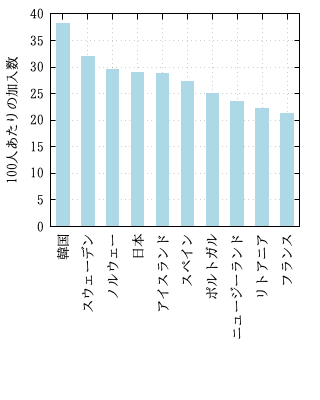
\includegraphics{fig.png}
    \caption{光ファイバー回線の加入者数(100人あたり)}\label{fig:fig1}
\end{figure}

% ーーー
% 節見出し(2)
\section{デジタル競争力ランキング}

% 本文(2)
国際経営開発研究所(IMD)の調査\cite{imd}によると,表\ref{tbl:tbl1}に示すように,日本のデジタル競争力のランキングは調査対象の64カ国中,総合で28位,知識分野で25位となっている.

% 表の挿入
% \begin{tabular}
% \end{tabular}    
% による表の記述を 
% \begin{table}[htbp]
% \end{table}
% で囲み
% \caption{}
% で表のタイトルを入れる.
% \label{}
% を使って表番号が参照できるようにする
% また,
% \centering
% で表が中央に来るようにする
\begin{table}[htbp]
    \centering
    \caption{デジタル競争力ランキング(64カ国中)}\label{tbl:tbl1}
    \begin{tabular}{|c|c|c|}\hline
        国 & 総合 & 知識 \\
        \hline
        米国 & 1位 & 3位 \\
        \hline
        香港 & 2位 & 5位 \\
        \hline
        スウェーデン & 3位 & 2位 \\
        \hline
        デンマーク & 4位 & 8位 \\
        \hline
        シンガポール & 5位 & 4位 \\
        \hline\hline
        韓国 & 12位 & 15位 \\
        \hline
        中国 & 15位 & 6位 \\
        \hline\hline
        日本 & 28位 & 25位 \\
        \hline
    \end{tabular}
\end{table}

% ーーー
% 見出し(3)
% 考察
%
% \begin{itemize}
% \end{itemize}
% を使って箇条書きで記述する
\section{考察}
\begin{itemize}
    \item 日本のブロードバンド普及率は高水準にある - OECD諸国の中で100人あたり約32-33の光ファイバー回線数を記録しており,デジタルインフラの基盤は充実している状況が読み取れます。
    \item デジタル競争力と基盤整備に乖離がある - ブロードバンド普及率は上位レベルにあるにも関わらず,IMDのデジタル競争力ランキングでは28位と中位に留まっており,インフラ以外の要因が競争力を制約している可能性があります。
    \item アジア諸国間での競争力格差が顕著 - 韓国(12位),中国(15位)と比較して日本(28位)は下位にあり,同じアジア地域でもデジタル活用や競争力に大きな差が生じています。
    \item 北欧諸国のデジタル競争力が突出している - デンマーク(1位),スウェーデン(3位)など北欧諸国が上位を占めており,これらの国々のデジタル政策や社会システムが参考になる可能性があります。
    \item 日本のデジタル化は量的整備から質的活用への転換点にある - 物理的なインフラは整備されているものの,それを効果的に活用したイノベーションや競争力向上に課題があることが示唆されており,デジタル化戦略の見直しが必要と考えられます。
\end{itemize}



% ここに参考文献が入る
%

\bibliographystyle{junsrt}
\bibliography{exercise.bib}

\end{document}